\section{Ensemble and Results}

\subsection{Final Ensemble}
The final model is an ensemble of three SANF-Net instances trained on the official training split with
different random seeds and identical settings. For each recording the class probabilities of the three
models are averaged and the most probable class is predicted. The ensemble has 429k parameters in total.

\subsection{Official Test Results}
Table~\ref{tab:main} compares SANF-Net with the published CEEDNet results on the official test split. The
ensemble reaches \textbf{72.9\% accuracy}, 72.3\% balanced accuracy, a macro F1 of 0.709 and a \textbf{macro AUC
of 0.870}. A single SANF-Net reaches $68.4\pm2.8\%$ (individual seeds 64.4\%, 70.3\% and 70.3\%). The ensemble
is above CEEDNet's best single model (70.2\%) and within 1.8 points of its nine-model ensemble (74.7\%), with
about 590 times fewer parameters. On the no-overlap subset, which excludes every patient seen in training, the
ensemble reaches 72.2\% (AUC 0.863), close to its full-test score, which indicates no leakage through repeated
patients. CEEDNet's ensemble reports 76.7\% on this subset. With 118 test recordings, the 95\% confidence
interval of any single test accuracy is about $\pm8$ points.

\begin{table}[H]
\centering
\caption{Three-class results on the official CAUEEG split (per recording). Single SANF-Net: mean $\pm$ s.d.\
over three seeds}
\label{tab:main}
\small
\begin{tabular}{lrcccccc}
\toprule
& & \multicolumn{4}{c}{Test ($n=118$)} & \multicolumn{2}{c}{No-overlap ($n=90$)}\\
\cmidrule(lr){3-6}\cmidrule(lr){7-8}
Model & Params & Acc & BAcc & F1 & AUC & Acc & AUC\\
\midrule
CEEDNet, best single model$^\dagger$ & 11M+ & 70.2 & -- & -- & -- & -- & --\\
CEEDNet, 9-model ensemble$^\dagger$ & 253.8M & 74.7 & -- & -- & -- & 76.7 & --\\
\midrule
SANF-Net, single & 143k & $68.4\pm2.8$ & $67.3\pm3.6$ & $.666\pm.035$ & $.849\pm.014$ & $67.4\pm1.4$ & $.844\pm.011$\\
\textbf{SANF-Net, 3-model ensemble} & 429k & \textbf{72.9} & \textbf{72.3} & \textbf{.709} & \textbf{.870} & \textbf{72.2} & \textbf{.863}\\
\bottomrule
\end{tabular}\\[2pt]
\parbox{\textwidth}{\scriptsize $^\dagger$As published by \citet{kim2023caueeg}, with their own training recipe and
test-time augmentation. Params: parameters; F1: macro F1.}
\end{table}

\textbf{Per-class performance.} Table~\ref{tab:perclass} gives the ensemble's confusion matrix and per-class
metrics. The model recognises 95.7\% of healthy participants and labels none of them as demented, and detects
77.4\% of dementia patients. MCI is the hardest class: its recall is 43.9\%, with errors split between the
two neighbouring classes, but its precision is the highest of all classes (75.0\%), so an MCI prediction is
usually correct. Severe errors (Normal predicted as Dementia or the reverse) are rare.

\begin{table}[H]
\centering
\caption{Confusion matrix (row percentages, counts in brackets) and per-class metrics of the SANF-Net ensemble
on the official test split}
\label{tab:perclass}
\small
\begin{tabular}{lccc@{\hspace{2em}}ccc}
\toprule
True $\downarrow$ / Predicted $\rightarrow$ & Normal & MCI & Dementia & Precision & Recall & F1\\
\midrule
Normal ($n=46$) & \textbf{95.7} (44) & 4.3 (2) & 0.0 (0) & 72.1 & 95.7 & .822\\
MCI ($n=41$) & 34.1 (14) & \textbf{43.9} (18) & 22.0 (9) & 75.0 & 43.9 & .554\\
Dementia ($n=31$) & 9.7 (3) & 12.9 (4) & \textbf{77.4} (24) & 72.7 & 77.4 & .750\\
\bottomrule
\end{tabular}
\end{table}

\textbf{What the model uses.} The mean modality gates on the test set differ by true class. For Normal
recordings the EEG branch has the largest weight (EEG 0.39, biomarkers 0.29, age 0.32); for MCI the biomarker
and age branches dominate (0.37 and 0.38, EEG 0.25); for Dementia the three are balanced (0.34, 0.35, 0.31).

\subsection{Cross-Validated Results}
Because a 118-recording test set is small and the official test split turns out to be easier than the pooled
data (the same models score $59.9\pm1.0\%$ on validation but $68.4\pm2.8\%$ on test), we also evaluate under
repeated five-fold cross-validation. SANF-Net reaches $59.5\pm0.3\%$ accuracy and a macro AUC of
$0.778\pm0.006$ over four fold assignments (first assignment: 59.8\%, 95\% CI 56.7--62.8\%), which is very stable
across repeats. Under the identical protocol it is significantly better than EEGNet ($+6.8$ points, CI
3.4--10.1) and better than the 1D-ResNet in AUC ($+0.028$, CI 0.003--0.050), and it is statistically
indistinguishable from logistic regression on the same normative biomarkers plus age (paired difference
$-0.1\pm0.5$ points). Out-of-fold recall is 76.8\% for Normal, 62.9\% for Dementia and 38.8\% for MCI
(Figure~\ref{fig:cm}). For MCI versus Normal the AUC is 0.787, detecting 63\% of MCI at 80\% specificity.

\begin{figure}[H]
\centering
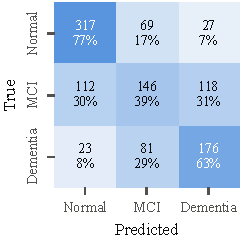
\includegraphics[width=0.45\textwidth]{figures/confusion.pdf}
\caption{SANF-Net out-of-fold confusion matrix under five-fold cross-validation ($n=1069$, counts and row
percentages).}
\label{fig:cm}
\end{figure}

\subsection{Ablation Study}
Table~\ref{tab:ablation} removes one component at a time under the same cross-validation protocol. Removing
both non-EEG branches clearly hurts: the EEG-only network loses 4.5 accuracy points (CI 1.4--8.0) and 0.049
macro AUC, and its MCI recall falls to 24.5\%. State-aware sampling gives a small but significant AUC gain
($+0.013$, CI 0.002--0.025), and normative scoring and the biomarker branch each add about 0.02 MCI-versus-Normal
AUC. Removing the ordinal head leaves accuracy and AUC unchanged but raises MCI recall from 38.8\% to 58.8\%,
at the cost of Normal and Dementia recall; this gives a screening-oriented operating point.

\begin{table}[H]
\centering
\caption{Ablations (five-fold cross-validation, out-of-fold, $n=1069$)}
\label{tab:ablation}
\small
\begin{tabular}{lcccc}
\toprule
Variant & Acc & AUC & AUC Normal vs MCI & MCI recall\\
\midrule
SANF-Net (full) & 59.8 & .780 & .787 & 38.8\\
\quad random crops, no state & 58.6 & .767 & .781 & 36.2\\
\quad no FiLM state conditioning & 58.9 & .777 & .784 & 41.8\\
\quad mean instead of attention pooling & 58.5 & .782 & .783 & 35.9\\
\quad plain standardisation (no normative) & 57.6 & .768 & .768 & 36.4\\
\quad no biomarkers & 57.3 & .772 & .767 & 34.8\\
\quad no age & 58.5 & .783 & .788 & 37.0\\
\quad EEG only & 55.3 & .731 & .719 & 24.5\\
\quad no ordinal head & 59.5 & .777 & .785 & 58.8\\
\bottomrule
\end{tabular}
\end{table}

\subsection{Protocol and Age Confounds}
Community-recruited normals differ from every other group in ways unrelated to cognition
(Table~\ref{tab:groups}, Figure~\ref{fig:protocol}): they are younger (61.7 versus 69.6--76.6 years), only 12\%
of their recordings include photic stimulation (versus 90--92\% of every other group), and their recordings
are shorter. A model can therefore recognise many community normals from the protocol alone.

\begin{figure}[H]
\centering
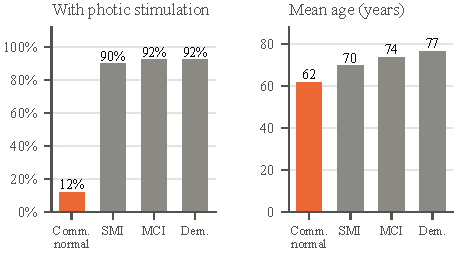
\includegraphics[width=0.7\textwidth]{figures/protocol.pdf}
\caption{Share of recordings with photic stimulation and mean age per subgroup. Community normals differ from
all clinical groups in both, independently of cognition.}
\label{fig:protocol}
\end{figure}

We therefore trained protocol-blind variants: (A) SANF-Net with photic segments and the three protocol
features removed, and (B) SANF-Net on eyes-closed segments only (Table~\ref{tab:confound}). Removing protocol
information costs SANF-Net 2.7 accuracy points and the linear model 2.5 points, almost entirely on the
community-versus-MCI comparison, whereas SMI-versus-MCI stays at 0.65--0.66 for every model. SANF-Net relies
less on the shortcut than the linear model, as its much higher SMI recall shows (57.9\% versus 35.7\%). After
1:1 age matching, SMI versus MCI falls to 0.54--0.57 for every model, and the 24 community normals recorded
with photic stimulation are not distinguished from age-matched MCI by any model (AUC 0.50--0.59).

\begin{table}[H]
\centering
\caption{Protocol confound (five-fold cross-validation, out-of-fold). Comm.: community-recruited normals
($n=229$); SMI: subjective memory impairment ($n=171$)}
\label{tab:confound}
\small
\begin{tabular}{lccccc}
\toprule
& & & \multicolumn{2}{c}{AUC vs MCI} & \\
\cmidrule(lr){4-5}
Model & Acc & AUC & Comm. & SMI & SMI recall\\
\midrule
Age (LR) & 51.1 & .709 & .858 & .618 & 42.7\\
Normative biomarkers + age (LR) & 59.3 & .778 & .951 & .655 & 35.7\\
\quad without protocol features & 56.8 & .747 & .863 & .660 & 50.6\\
SANF-Net & 59.8 & .780 & .891 & .653 & 57.9\\
\quad (A) no photic information & 57.1 & .764 & .852 & .649 & 63.7\\
\quad (B) eyes-closed only & 58.5 & .756 & .842 & .650 & 63.7\\
\bottomrule
\end{tabular}
\end{table}

\subsection{External Validation}
Table~\ref{tab:external} reports MCI-versus-normal performance on the external cohorts without retraining, using
the five cross-validation fold models (predictions averaged); MCI is scored with $1-P(\text{Normal})$. Since age
is uninformative there, these results reflect EEG and biomarkers only. We also apply a label-free \emph{site
calibration}: channel amplitudes are rescaled to the cohort's median and the normative $z$-scores are
re-centred on the cohort's own normals in a leave-one-out manner. On the pooled Isfahan cohorts the AUC is
0.67, rising to \textbf{0.70} with site calibration (0.76 on Isfahan 2016); on GENEEG, whose montage and
protocol differ more, it is 0.58. Across the external cohorts 81--91\% of healthy participants are correctly
classified as Normal. With 61--63 subjects per cohort all intervals are wide.

\begin{table}[H]
\centering
\caption{External MCI versus normal without retraining. AUC with 95\% bootstrap confidence interval}
\label{tab:external}
\small
\begin{tabular}{lccc}
\toprule
Cohort & $n$ (MCI) & No calibration & Site calibration\\
\midrule
Isfahan 2016 & 27 (11) & .73 (.51--.91) & .76 (.57--.92)\\
Isfahan 2019 & 34 (18) & .64 (.45--.84) & .63 (.44--.81)\\
Isfahan pooled & 61 (29) & .67 (.53--.80) & .70 (.56--.83)\\
GENEEG & 63 (28) & .58 (.44--.72) & .58 (.42--.74)\\
\bottomrule
\end{tabular}
\end{table}

\begin{figure}[H]
\centering
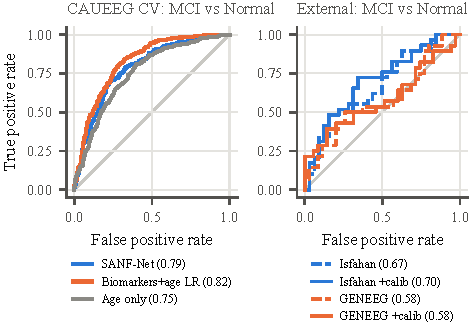
\includegraphics[width=0.85\textwidth]{figures/roc.pdf}
\caption{MCI versus normal ROC curves. Left: CAUEEG out-of-fold predictions. Right: external cohorts without
retraining, with and without site calibration.}
\label{fig:roc}
\end{figure}
